%%%%%%%%%%%%%%%%%%%%%%%%%%%%%%%%%%%%%%%%%%%%%%%%%%%%%%%%%%%%%%%%%%%%%%%%%
%                                                                       
%                                                                       
%    A latex template for ATMS PhD preliminary examination proposal.    
%                          Created by Xiaotian Xu, Jan/25/2024          
%                                     xx24@illinois.edu                 
%               Feel free to contact me if you have any porblem.        
%                                                                       
%                                                                       
%%%%%%%%%%%%%%%%%%%%%%%%%%%%%%%%%%%%%%%%%%%%%%%%%%%%%%%%%%%%%%%%%%%%%%%%%
\documentclass[11pt]{article} % 11 font size
\usepackage{newtxtext,newtxmath} % Times font
\usepackage{setspace} % Provides support for setting the spacing between lines. Required for \singlespacing below
\usepackage{graphicx} % Required for including graphics in your document.
\usepackage{geometry} % Used for adjusting page dimensions and margins. Set up A4 paper with 1 inch margin.
\geometry{a4paper,left=1in,right=1in,top=1in,bottom=1in}
\usepackage{tocloft} % Customizes the appearance of the table of contents, list of figures, and list of tables.
\usepackage{amsmath} % Enhances LaTeX's math capabilities. Essential for writing complex mathematical equations, aligning equations.
\usepackage[round, authoryear]{natbib} % Required for bibliographies and citations. 
\usepackage{varwidth} % Allows the creation of minipages of variable width, useful for boxes that shrink to the natural width of their contents.
\usepackage{enumitem} % Provides control over the layout of itemize, enumerate, description, and list environments.
\usepackage{color} % Provides support for color
\usepackage{algorithm} % Used to write algorithms in a structured format.
\usepackage{algorithmic} % Used in conjunction with the algorithm package.
\usepackage{nameref} % Allows you to reference section names, captions, etc., in your document by their label.
% \usepackage{hyperref} % For hyperlinks within the paper and references. Help you easily find refs while writing your draft. 
\usepackage{makecell} % Provides flexible macros to format table cells.
\usepackage{float} %  Improves the interface for defining floating objects such as figures and tables. 
\usepackage[modulo]{lineno} % Adds line numbers to your document. The modulo option displays only line numbers that are multiples of five.
\usepackage{fancyhdr} % Enhances LaTeX's capabilities for handling page headers and footers, allowing for easy customization.
\usepackage{tabularx} % Enhances the quality of tables in LaTeX, providing an additional column type. 

% Increase the space for section numbers and adjust the indentation
\setlength{\cftsecnumwidth}{3em} % Adjust the width as needed
\setlength{\cftsubsecnumwidth}{3.5em} % Adjust the width as needed
\setlength{\cftsubsecindent}{\cftsecnumwidth}
\setlength{\cftsubsubsecnumwidth}{4em} % Adjust the width as needed
\setlength{\cftsubsubsecindent}{\dimexpr\cftsubsecnumwidth+\cftsubsecindent\relax}


\begin{document}
\singlespacing
\pagenumbering{gobble} % Remove page numbering for the first page

\parbox[t][2cm][c]{\textwidth}{\LARGE
    \begin{center} \textsc{University of Illinois Urbana-Champaign} \end{center}}

\parbox[t][1cm][c]{\textwidth}{\Large
    \begin{center} \textsc{Proposal For Ph.D. Preliminary Exam}\end{center}}

\parbox[t][1cm][c]{\textwidth}{\large
    \begin{center} \textsc{Department of Atmospheric Sciences}\end{center}}
\\
\\
\\
\parbox[t][9cm][c]{\linewidth}{%
    \raisebox{-0.5\height}{\rule{\linewidth}{2pt}}
    \huge \begin{center} {\textbf{Title}}\end{center}
    \raisebox{0.5\height}{\rule{\linewidth}{2pt}}}
\\
\\
\\
\textit{Author:} \hfill \textit{Committee members:}\\
\noindent
\begin{minipage}[t]{0.4\textwidth}
  first name \textsc{last name}
\end{minipage}%
\hfill
\begin{minipage}[t]{0.6\textwidth}
  \raggedleft
  Prof. first name \textsc{last name} \\
  Prof. first name \textsc{last name} \\
  Prof. first name \textsc{last name} \\
  Prof. first name \textsc{last name}
\end{minipage}
\\
\\
\\
\\
\\
\\
\\
\\
\centerline{\today}

\newpage
\pagestyle{fancy}
\fancyhf{} % Clear header and footer
\rfoot{\thepage} % Page number in the right bottom corner
\renewcommand{\headrulewidth}{0pt} % Remove header horizontal line
\pagenumbering{arabic} % Start page numbering from "Project summary" page
\setcounter{page}{1} % Set page number to 1

\noindent \textbf{\Huge Project summary \textbf{\color{red} (1 page limitation)}} \\
\\
Write your project summary here.  \par

\newpage
% Customizations for the table of contents
\renewcommand{\contentsname}{\Huge\textbf{Contents}\textbf{\color{red} (1 page limitation)}\\}
\renewcommand{\cfttoctitlefont}{\Huge\textbf}
\renewcommand{\cftaftertoctitle}{\hfill}
\renewcommand{\cftsecfont}{\normalsize}
\renewcommand{\cftsubsecfont}{\normalsize}
\renewcommand{\cftsubsubsecfont}{\normalsize}
\renewcommand{\cftsecpagefont}{\normalsize\bfseries}
\renewcommand{\cftsubsecpagefont}{\normalsize\bfseries}
\renewcommand{\cftsubsubsecpagefont}{\normalsize\bfseries}
\renewcommand\thesection{\Roman{section}}
\renewcommand\thesubsection{\Roman{section}.\Alph{subsection}}
\renewcommand\thesubsubsection{\Roman{section}.\Alph{subsection}.\arabic{subsubsection}}
\tableofcontents
\thispagestyle{fancy}

\newpage
\linenumbers
\section{Introduction}
\textbf{\color{red} Introduction should includes general motivation for proposed research.}
\subsection{University}
The University of Illinois at Urbana Champaign is a public land-grant research university founded in 1867. \par

\subsection{College}
The College of Liberal Arts and Sciences (LAS) is the largest college of the University of Illinois Urbana-Champaign.

\subsection{Department}
The Department of Atmospheric Science had its beginnings in 1969 with the arrival of Professor Yoshimitsu Ogura to the University of Illinois campus. 

The Doppler on Wheels (DOW) mobile radar (Figure \ref{fig:dow}) and instrumentation facility has joined the Department of Atmospheric Sciences at the University of Illinois at Urbana-Champaign.\par
\begin{figure}[h]
    \centering
    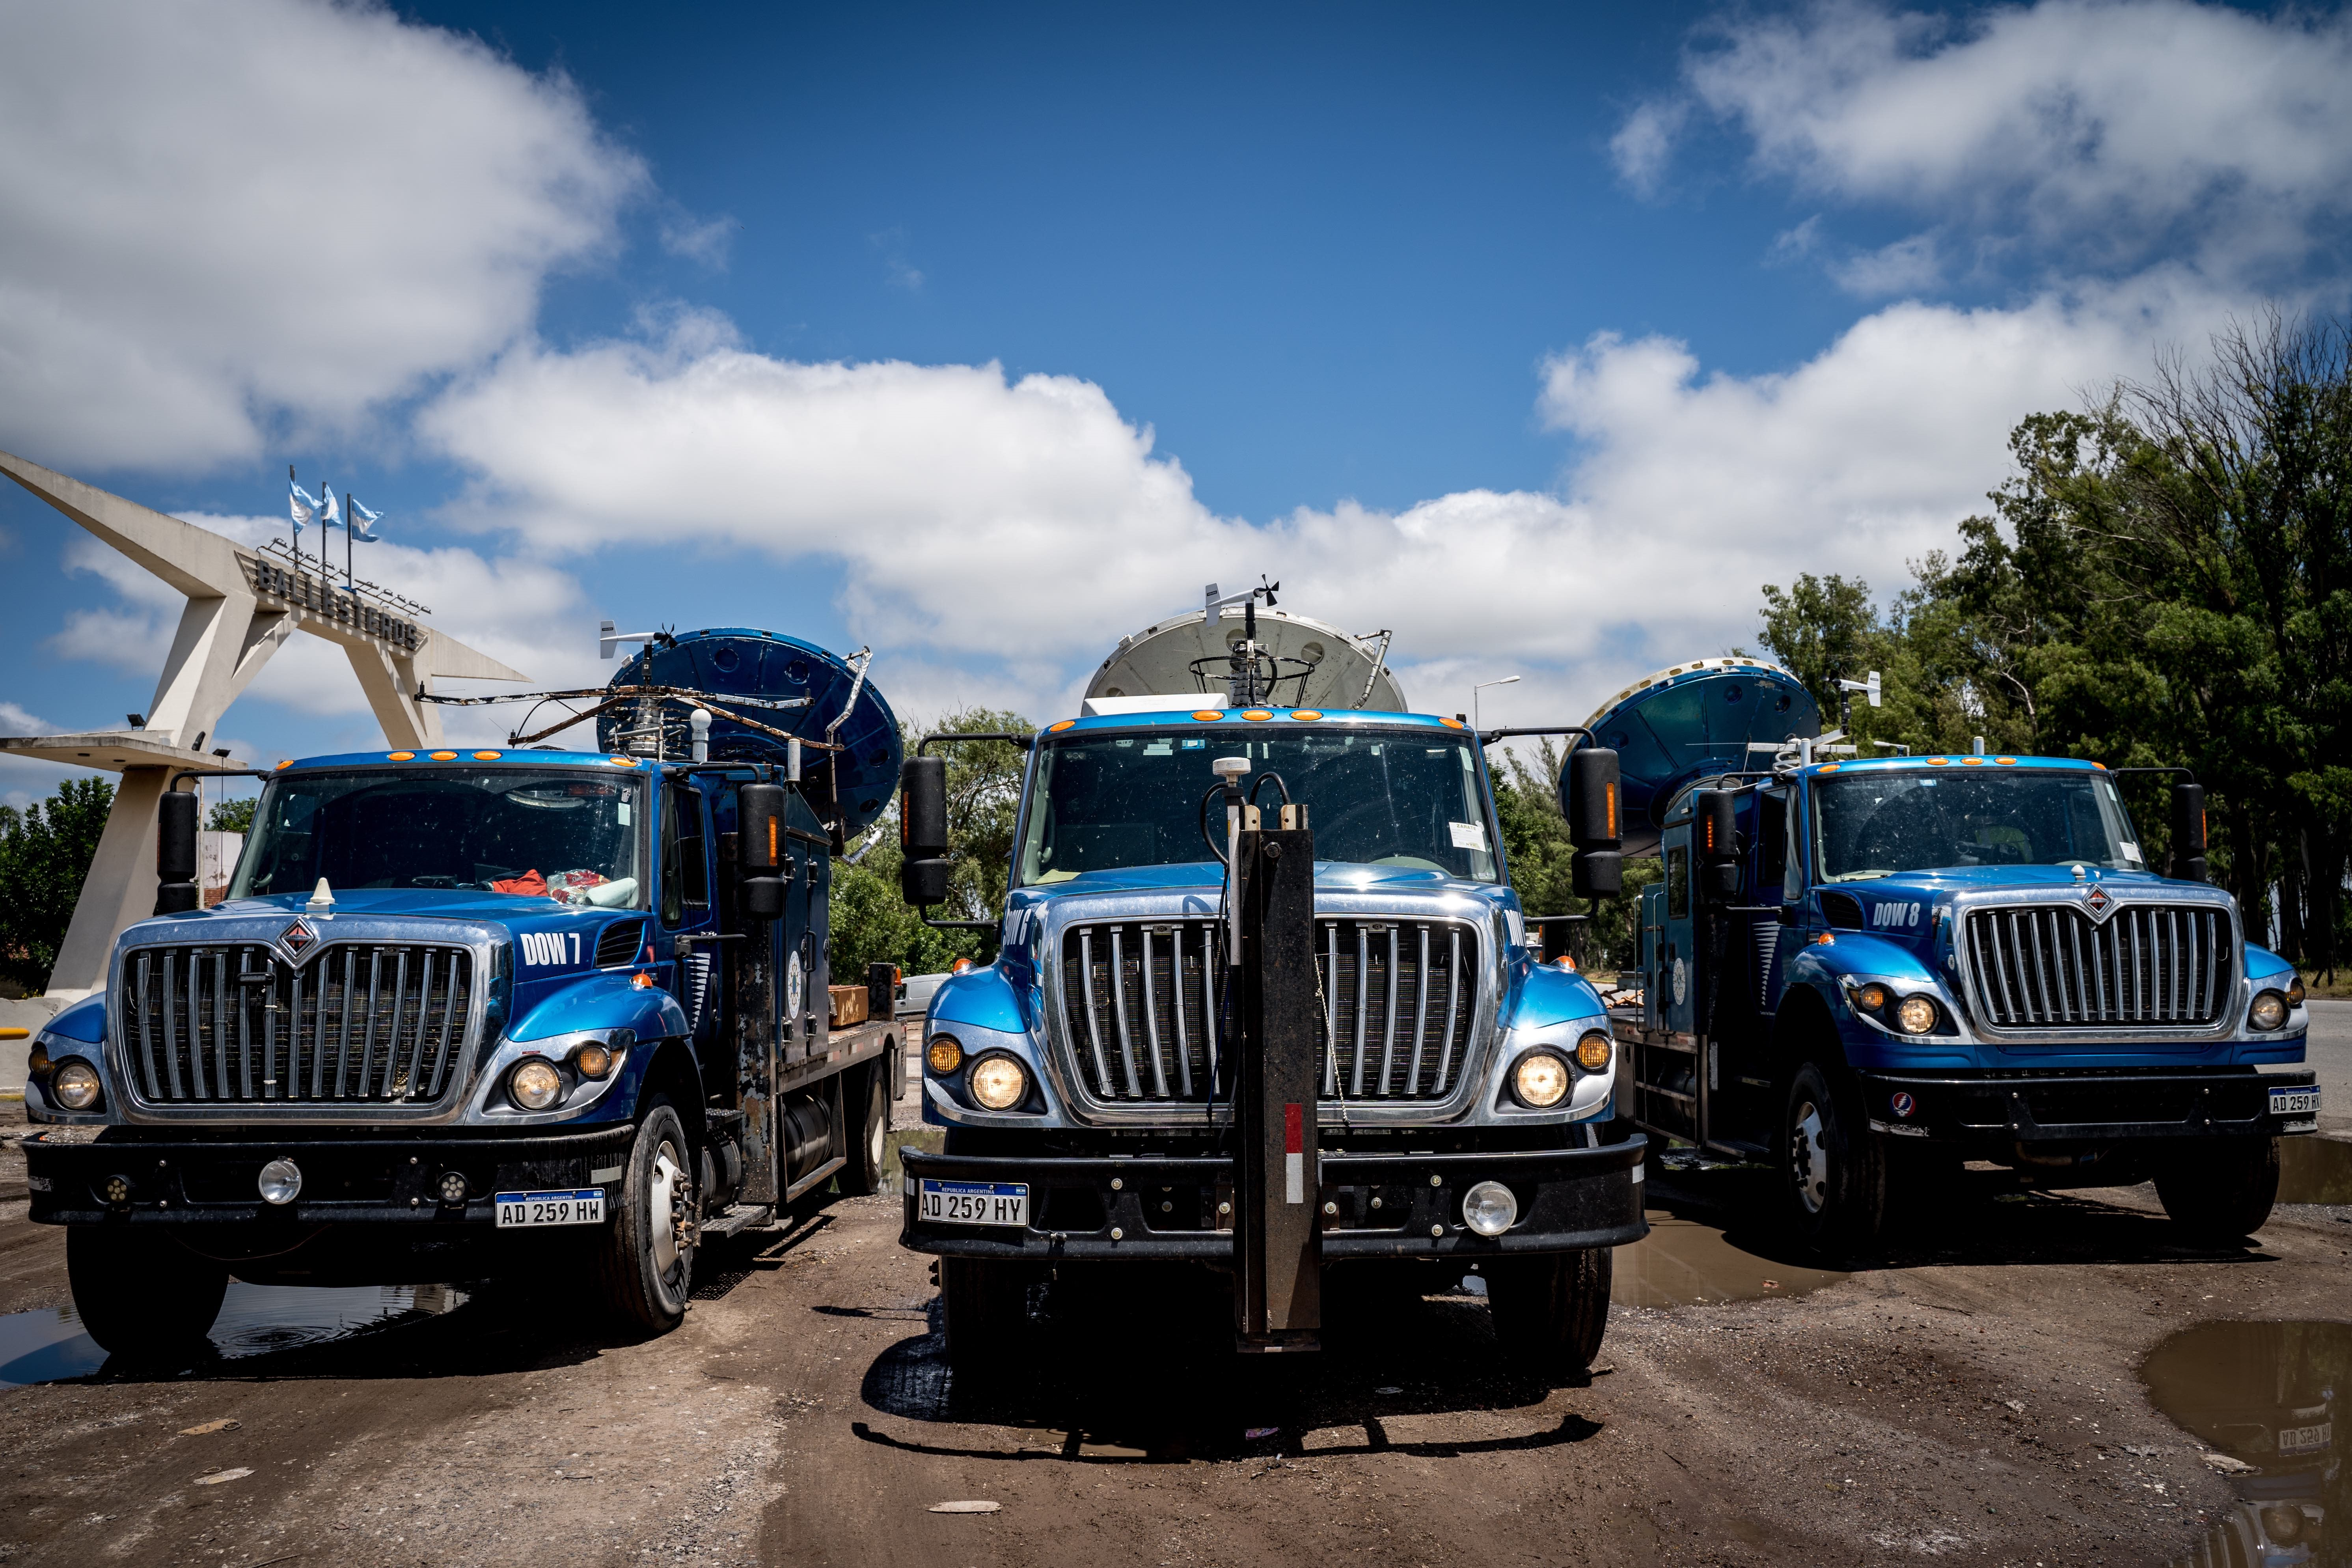
\includegraphics[width=0.5\textwidth]{DOW.jpg}
    \caption{DOW.}
    \label{fig:dow}
\end{figure}

There are many research work based on DOW \citep{wurman2021flexible,juliano2023toward}. \citet{wurman2021flexible} describes xxxx. 

\section{Objectives/Hypotheses}
\textbf{\color{red}Objectives should include their relationship to the current state of knowledge and to any relevant preliminary results for the proposed research.}
Our objective is to investigate xxxxxx. \par

\section{Proposed research}
\textbf{\color{red} Proposed research should include methodology and its relationship to achieving stated objectives and answering proposed hypotheses.}
\subsection{Task 1:xxxxx.}
Task 1 prepare to xxxxxx .\par
\vspace{\baselineskip}
\noindent \textbf{Task 1A: xxxxxx.}
Task 1A focus on xxxxxx. \par
\vspace{\baselineskip}
\noindent \textbf{Task 1B: xxxxxx.}
Task 1B plans to xxxxxx.  \par

\subsection{Task 2:xxxxx.}
Task 2 prepare to xxxxxx .\par
\vspace{\baselineskip}
\noindent \textbf{Task 2A: xxxxxx.}
Task 2A focus on xxxxxx. \par
\vspace{\baselineskip}
\noindent \textbf{Task 2B: xxxxxx.}
Task 2B plans to xxxxxx.  \par

\section{Preliminary work}
The work we have currently finished is divided into several parts. \par
% Label each each section, figure, table can help you easily cite them later.
\subsection{XXXXXX}\label{sec:first_work}
What we have done is to derive the thermodynamic equation which is shown in equation [\ref{thermo}].
\begin{equation}\label{thermo} 
	C_v\frac{\mathrm{d} T}{\mathrm{d} t}+p\frac{\mathrm{d} \alpha }{\mathrm{d} t} =Q ,
\end{equation}
where $C_v$ is xxx, $T$ is xxxx. \par

We will continue working on xxxx. We will continue working on xxxx. We will continue working on xxxx. We will continue working on xxxx. \par
We will continue working on xxxx. We will continue working on xxxx. We will continue working on xxxx. We will continue working on xxxx. \par
We will continue working on xxxx. We will continue working on xxxx. We will continue working on xxxx. We will continue working on xxxx. \par

\subsection{XXXXXX}\label{sec:second_work}
Section \ref{sec:first_work} introduces xxxx, the second work we have don is to derive equation [\ref{momen}]. 
% There are several ways to create equations that you want, here is a website you could learn it. https://docs.aspose.com/tex/java/latex-structures-for-equations/
% An alternative methods is to use Latex online equation editor (e.g. https://www.tutorialspoint.com/latex_equation_editor.htm) and copy the code here.
\begin{equation}\label{momen}
	\left. \begin{aligned}
		fv-\frac{1}{\rho}\frac{\partial p}{\partial x} = & \frac{\mathrm{d} u}{\mathrm{d} t}\\
		-fu-\frac{1}{\rho}\frac{\partial p}{\partial y} = &\frac{\mathrm{d} v}{\mathrm{d} t}\\
		-g-\frac{1}{\rho}\frac{\partial p}{\partial z} = &\frac{\mathrm{d} w}{\mathrm{d} t},\\
	\end{aligned}
	\right \}
\end{equation}
where $f$ is xxxx. \par

We will continue working on xxxx. We will continue working on xxxx. We will continue working on xxxx. We will continue working on xxxx. \par
We will continue working on xxxx. We will continue working on xxxx. We will continue working on xxxx. We will continue working on xxxx. \par
We will continue working on xxxx. We will continue working on xxxx. We will continue working on xxxx. We will continue working on xxxx. \par

\section{Work plan}
\textbf{\color{red} Work Plan should include timetable and justification for any computer time needed.}\\
\begin{tabularx}{\textwidth}{lXXX}
	& \textbf{Task 1} & \textbf{Task 2} & \arraybackslash\textbf{Task 3} \\
	\hline
	\hline
	\textbf{Summer 2023} & Finish Task 1 &  &  \\ 
	\hline
	\textbf{Fall 2023} & Write paper 1 & Start Task 2 &  \\
	\hline
	\textbf{Spring 2024} & Finish paper 1 & \makecell[l]{Finish Task 2 \\ Write paper 2} &  \\
	\hline
	\textbf{Summer 2024} & & Finish paper 2 & Start task 3 \\ 
	\hline
	\textbf{Fall 2024} & & & \makecell[l]{Finish Task 3 \\ Write paper 3}\\
	\hline
	\textbf{Spring 2025} & & & Finish paper 3  \\
	\hline
	\multicolumn{1}{l}{\textbf{Summer \& Fall 2025}} & \multicolumn{3}{c}{Write thesis \& Finish thesis} \\
	\hline
\end{tabularx}
\\
\\
\\
\\
\\
\\
\\
\\
\textbf{\huge \color{red} Maximum 15 pages excluding cover page, biography and references}

\newpage
\section{Biography}
\textbf{Your Name} \\
Graduate Research Assistant, Department of Atmospheric Science \\
University of Illinois Urbana Champaign \\
1301 W Green St, Urbana, IL, 61801 \\
your email@illinois.edu \\
\\
\noindent \textbf{Education} 
\begin{itemize}[leftmargin=0.2in, itemsep=-0.5em]
    \item Sep. 2022 $-$ present, Ph.D. studet, Atmospheric Science, University of Illinois Urbana-Champaign
    \item Sep. 2018 $-$ Jun. 2022, B.Sc., Atmospheric Science, University of Illinois Urbana-Champaign
\end{itemize} 

\noindent \textbf{Publications}
\begin{itemize}[leftmargin=0.2in, itemsep=-0.5em]
    \item xxxx 
    \item xxxx
    \item xxxx
    \item xxxx
    \item xxxx
\end{itemize}

\noindent \textbf{Presentations}
\begin{itemize}[leftmargin=0.2in, itemsep=-0.5em]
    \item Talk, xxxx
    \item Poster, xxxx
\end{itemize}

% Set up reference
\newpage
\section{Reference}
\renewcommand{\bibsection}{}
\renewcommand{\bibfont}{\small}
\bibliographystyle{apalike}
\setlength{\bibsep}{0pt}
\bibliography{main}

\end{document}

